% "{'classe':('PSI'),'chapitre':'dyn_pfd_vehicule','type':('application'),'titre':'Conducteur virtuel pour véhicule automobile', 'source':' Centrale Supélec PSI 2014','comp':('C1-05','C2-09'),'corrige':True}"
%\setchapterimage{bandeau}
\chapter*{Application \arabic{cptApplication} \\ 
Conducteur virtuel pour véhicule automobile -- \ifprof Corrigé \else Sujet \fi}
\addcontentsline{toc}{section}{Application \arabic{cptApplication} : Conducteur virtuel pour véhicule automobile -- \ifprof Corrigé \else Sujet \fi}

\iflivret \stepcounter{cptApplication} \else
\ifprof  \stepcounter{cptApplication} \else \fi
\fi

\setcounter{question}{0}
\marginnote{Centrale Supélec PSI 2014.}
\marginnote[1cm]{
\UPSTIcompetence[2]{C1-05}
\UPSTIcompetence[2]{C2-09}
}
\begin{marginfigure}[4cm]
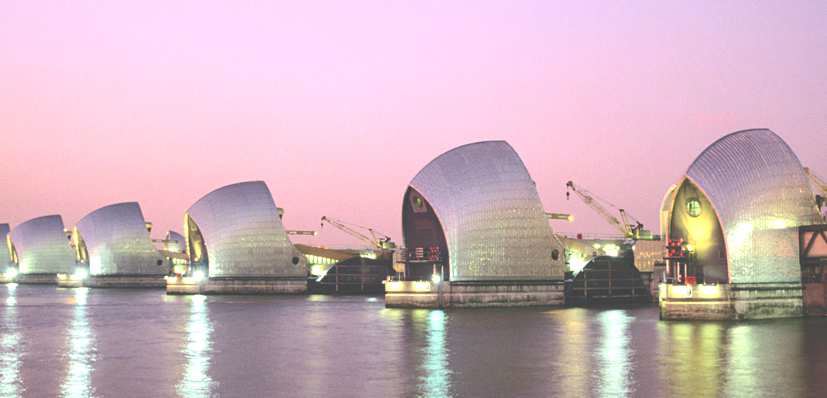
\includegraphics[width=\linewidth]{fig_00}
\end{marginfigure}




\ifprof
\else
L'accroissement de la circulation automobile dans les grandes agglomérations
menace de saturation leur réseau d'autoroutes. Une des solutions consiste à
augmenter les flux en automatisant les voitures sur ces dernières. Après une
évaluation du gain en terme de flux d'automobiles que peut apporter ce concept,
l'étude portera sur le système de guidage automatique latéral d'une automobile
sur une autoroute dite «~intelligente~».
\fi


\begin{obj}
L'objet de cette partie est de déterminer un modèle mécanique du véhicule en
appliquant les théorèmes généraux de la dynamique au véhicule . L'idée est
d'utiliser un modèle mécanique relativement simple, associé à une commande
très robuste.
\end{obj}

%\begin{center}
%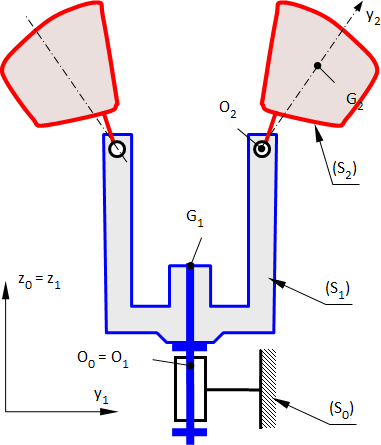
\includegraphics[width=.5\linewidth]{fig_02}
%\end{center}


\ifprof
\else
Une approche simplifiée permettant d'aborder le problème consiste à adopter un
modèle dit « bicyclette », représenté sur la figure suivante, qui assimile le comportement
du véhicule à celui d'une bicyclette :
\begin{itemize}
\item le train avant directeur se réduit à une seule roue (12) sur laquelle s’appliquent
les actions exercées sur les deux roues avant (1) et (2) du véhicule, de
même la roue arrière (34) supporte les actions exercées par l’essieu arrière
portant les roues (3) et (4), les pneumatiques avant et arrière
ont les mêmes caractéristiques, en particulier le même coefficient de dérive
(celui-ci sera défini plus loin);
\item le modèle choisi est un modèle à 2 degrés de liberté : l’angle de lacet
$\psi(t)=\angl{X_g}{X_L}$ et l’angle d’attitude $\alpha(t)=\angl{X_L}{U}$. La rotation de chaque
roue autour de son axe n’est pas prise en compte;
\item on notera que l’angle de braquage des roues $\beta(t)=\angl{X_L}{X_W}$ avant est
imposé au moyen d’un asservissement qui ne sera pas étudié dans le cadre
de ce problème;
\item les roues ont une masse supposée négligeable.
\end{itemize}
Cette modélisation ne prend pas en compte les mouvements suivants : tangage
(rotation autour de $\vect{Y_L}$) et roulis (rotation autour de $\vect{X_L}$).



\begin{marginfigure}
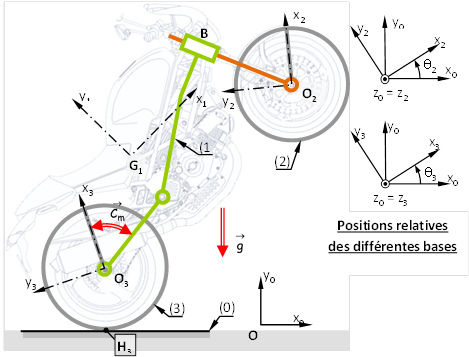
\includegraphics[width=\linewidth]{fig_01.png}
\end{marginfigure}

Les différents repères sont les suivants : 
\begin{itemize}
\item repère galiléen : $\rep{g} \repere{O_R}{X_g}{Y_g}{Z_g}$, $O_R$ est lié à la route, $\Pi_R = \angl{X_g}{Y_g}$ plan fixe par rapport à la route;
\item repère intermédiaire : $\rep{1} \repere{O_1}{X_g}{Y_g}{Z_g}$, $\vect{O_R O_1} = a \vect{Y_g}$ ;
\item repère intermédiaire : $\rep{0} \repere{O}{X_g}{Y_g}{Z_g}$, $O$ lié au châssis et $\vect{O_1 O} = b \vect{X_L}$, $\vecto{\rep{0}}{\rep{g}}=\vect{0}$, $\vectv{O}{\rep{0}}{\rep{g}}=V\vect{U}$ avec $\vect{O_R O}\cdot \vect{Z_g}=0$ 
et $V$ constante positive;
\item repère lacet $\rep{0} \repere{G}{X_L}{Y_L}{Z_L}$, $\vect{OG}=h\vect{Z_g}$ avec $G$ centre d'inertie lié du châssis  
lié au véhicule, $\vect{Z_L}=\vect{Z_g}$ et $\angl{Y_g}{Y_L}=\angl{X_g}{X_L}=\psi(t)$ angle de lacet, $h$ constate positive;
\item repère lié à la roue $\rep{W} \repere{A_i}{X_W}{Y_W}{Z_W}$, $A_i$ centre de la roue $R_i$ (assimilée à un disque), $\vect{Z_W}=\vect{Z_L}$ avec $\vect{OA_{12}}=l_1\vect{X_L}$ et $\vect{OA_{34}}=-l_2\vect{X_L}$, $\angl{Y_L}{Y_W}=\angl{X_L}{X_W}=\beta(t)$ angle de braquage.
\end{itemize}

On appelle :
\begin{itemize}
\item $\alpha(t)=\angl{X_L}{U}$ : angle d’attitude,
\item $\psi(t)=\angl{X_G}{X_L}$ : angle de lacet,
\item $\beta(t)=\angl{X_L}{X_W}$ : angle de braquage de la roue avant.
\end{itemize}
Le torseur cinématique du mouvement du véhicule (VH) par rapport à $\rep{g}$, au
point $O$, est noté :
$\torseurcin{V}{\text{VH}}{\rep{g}}=\torseurl{\vecto{\text{VH}}{\rep{g}}}{\vectv{O}{\text{VH}}{\rep{g}}=V\vect{U}}{O}$.


\begin{marginfigure}
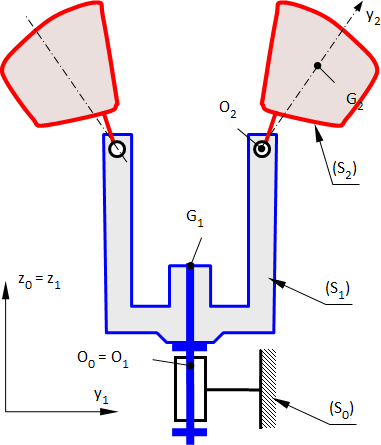
\includegraphics[width=\linewidth]{fig_02.png}
\end{marginfigure}
La roue munie d’un pneumatique se comporte différemment d’une roue rigide au niveau du contact avec le sol.
On adoptera le modèle représenté sur la figure ci-contre.

Le contact roue/sol pour chaque roue est modélisé par le torseur d’efforts
suivant :
$\torseurstat{T}{\text{Sol}}{\rep{i}}=\torseurl{\vectf{\text{Sol}}{\rep{i}} }{\vectm{M_i}{\text{Sol}}{\rep{i}}}{M_i} $ avec  $i\in\{12,34\}$ avec $\vect{OM_{12}}=\ell_1\vect{X_L}-R\vect{Z_L}$ et $\vect{OM_{34}}=-\ell_2\vect{X_L}-R\vect{Z_L}$.


L’angle de dérive d’un pneumatique est défini par : $\delta_i=\left(\vect{X_W},\vect{V\left(M_i / \rep{g} \right)}\right)$. Si
$D$ désigne le coefficient de dérive du pneumatique, on admettra qu’on peut écrire $Y_i = - D\delta_i$, soit ici $Y_{12}=-2D\delta_{12}$ et $Y_{34}=-2D\delta_{34}$.
Comme la vitesse du véhicule est supposée constante et la roue arrière n’est pas motrice, on peut considérer : $X_{12}=0$ et $X_{34}=0$.
La matrice d’inertie du véhicule de masse $M$, dans le repère $\rep{L}$, est de la
forme : $\inertie{G}{\text{VH}}=\matinertie{A}{B}{C}{0}{-E}{0}{\rep{L}}$
Remarque : le véhicule comprend la caisse, les roues, et sera modélisé
dans la mise en équation comme un solide indéformable.
\fi

\subsection*{Modélisation du comportement dynamique du véhicule}

\question{Déterminer les composantes dans le repère $\rep{L}$ du moment cinétique
$\vectmc{O}{\text{VH}}{\rep{g}}$ au point $O$, du véhicule (VH) dans son mouvement par rapport au repère $\rep{g}$, en fonction de $\dot{\psi}$, $\alpha$, $h$, $V$ et des caractéristiques inertielles.}
\ifprof
\begin{corrige}

La matrice d'inertie étant donnée en $G$, commençons par calculer 
$\vectmc{G}{\text{VH}}{\rep{g}} = \inertie{G}{\text{VH}} \vecto{\text{VH}}{\rep{g}} $
$ =\matinertie{A}{B}{C}{0}{-E}{0}{\rep{L}} \dot{\psi}\vect{Z_g} $
$ =\matinertie{A}{B}{C}{0}{-E}{0}{\rep{L}} \begin{pmatrix} 0 \\ 0 \\ \dot{\psi} \end{pmatrix}_{\rep{L}} $
$ =  \begin{pmatrix} -E\dot{\psi} \\ 0 \\ C\dot{\psi} \end{pmatrix}_{\rep{L}} $.

Il faut alors déplacer le moment cinétique. On aura pour cela besoin de $\vectv{G}{\text{VH}}{\rep{g}} $
$= \vectv{O}{\text{VH}}{\rep{g}} + \vect{GO}\wedge  \vecto{\text{VH}}{\rep{g}}$
$ = V\vect{U}-h\vect{Z_g} \wedge  \dot{\psi}\vect{Z_g} $
$ = V\vect{U}$.

Au final, 
$\vectmc{O}{\text{VH}}{\rep{g}} =\vectmc{G}{\text{VH}}{\rep{g}} +\vect{OG}\wedge MV\vect{U}$
$ = \begin{pmatrix} -E\dot{\psi} \\ 0 \\ C\dot{\psi} \end{pmatrix}_{\rep{L}} + h\vect{Z_g} \wedge MV\vect{U}$ 
$ = \begin{pmatrix} -E\dot{\psi} \\ 0 \\ C\dot{\psi} \end{pmatrix}_{\rep{L}} + hMV\vect{V}$ 
$ = \begin{pmatrix} -E\dot{\psi} \\ 0 \\ C\dot{\psi} \end{pmatrix}_{\rep{L}} + hMV\left(\cos\alpha \vect{Y_L} - \sin\alpha \vect{X_L} \right)$ 
$ = \begin{pmatrix} -E\dot{\psi} - hMV \sin\alpha \\ hMV\cos\alpha \\ C\dot{\psi} \end{pmatrix}_{\rep{L}} $.

\textbf{ -- Je note $\vect{V}$ le vecteur tel que $\base{U}{V}{Z_L}$ est une base. --}
\end{corrige}
\else
\fi

\question{Déterminer les composantes dans le repère $\rep{L}$ du moment dynamique
$\vectmd{O}{\text{VH}}{\rep{g}}$
au point $O$, du véhicule (VH) dans son mouvement par rapport au
repère $\rep{g}$, en fonction de $\dot{\psi}$, $\ddot{\psi}$, $\dot{\alpha}$, $\alpha$, $h$, $V$ et des caractéristiques inertielles.
}\ifprof
\begin{corrige} ~\\

On a en un point quelconque
 $\vectmd{O}{\text{VH}}{\rep{g}} =\left[ \dfrac{\dd \vectmc{O}{\text{VH}}{\rep{g}}}{\dd t}\right]_{\rep{g}}+\vectv{O}{\text{VH}}{\rep{g}} \wedge M\vectv{G}{\text{VH}}{\rep{g}}$.
 
 D'une part, $\left[ \dfrac{\dd \vect{X_L} }{\dd t}\right]_{\rep{g}} = \dot{\psi}\vect{Y_L}$ et $\left[ \dfrac{\dd \vect{Y_L} }{\dd t}\right]_{\rep{g}} = -\dot{\psi}\vect{X_L}$. On a donc 
 $\left[ \dfrac{\dd \vectmc{O}{\text{VH}}{\rep{g}}}{\dd t}\right]_{\rep{g}} $ 
 
 $ = 
  \begin{pmatrix} 
  -E\ddot{\psi} - \dot{\alpha} hMV \cos\alpha - \dot{\psi}\left( hMV\cos\alpha\right)\\ 
  -\dot{\alpha} hMV\sin\alpha +\dot{\psi}\left( -E\dot{\psi} -  hMV \sin\alpha\right)\\ 
  C\ddot{\psi} \end{pmatrix}_{\rep{L}} 
  $.
  
  D'autre part, $\vectv{O}{\text{VH}}{\rep{g}} \wedge M\vectv{G}{\text{VH}}{\rep{g}}$ $=V\vect{U}\wedge MV\vect{U} = \vect{0}$.
  
  Au final, $\vectmd{O}{\text{VH}}{\rep{g}} = \begin{pmatrix} 
  -E\ddot{\psi} - \left(\dot{\alpha} + \dot{\psi}\right( hMV\cos\alpha)\\ 
  -E\dot{\psi}^2 -\left(\dot{\alpha} +\dot{\psi}\right)  hMV \sin\alpha\\ 
  C\ddot{\psi} \end{pmatrix}_{\rep{L}} 
  $.

\end{corrige}
\else
\fi
\question{On note $\vect{\Gamma\left(G/\rep{g} \right)}$ le vecteur accélération de appartenant à $(\text{VH})$
dans son mouvement par rapport au référentiel galiléen $\rep{G}$. Déterminer $\vect{\Gamma\left(G/\rep{g} \right)}\cdot \vect{Y_L}$
en fonction de $\dot{\psi}$, $\dot{\alpha}$, $\alpha$, $V$. Linéariser la relation obtenue au voisinage
de la position d'équilibre définie par $\alpha=0$, $\psi=0$ et $\beta=0$.}
\ifprof
\begin{corrige}
On a vu que $\vectv{G}{\text{VH}}{\rep{g}} = V\vect{U}$, donc  $\vectg{G}{\text{VH}}{\rep{g}} = V\left(\dot{\psi}+\dot{\alpha} \right)\vect{V}$
$= V\left(\dot{\psi}+\dot{\alpha} \right)\left( \cos\alpha \vect{Y_L} - \sin\alpha \vect{X_L} \right)$. 
On a donc  $\vect{\Gamma\left(G/\rep{g} \right)}\cdot \vect{Y_L} = V\left(\dot{\psi}+\dot{\alpha} \right) \cos\alpha  $.
En linéarisant cette relation, on a  $\vect{\Gamma\left(G/\rep{g} \right)}\cdot \vect{Y_L} = V\left(\dot{\psi}+\dot{\alpha} \right)$.

\end{corrige}
\else
\fi


\question{En admettant que l’angle de dérive de la roue avant s’écrit : $\delta_{12}\simeq\alpha-\beta+\dfrac{\ell_1}{V}\dot{\psi}$ et celui de la roue arrière $\delta_{34}\simeq\alpha-\dfrac{\ell_2}{V}\dot{\psi}$, en déduire l’expression de $\vectf{\overline{\text{VH}}}{\text{VH}}\cdot \vect{Y_L}$. Linéariser la relation obtenue au voisinage
de la position d'équilibre définie par $\alpha=0$, $\psi=0$ et $\beta=0$.}
\ifprof
\begin{corrige}
On a $Y_{12}=-2D\delta_{12}$ et $Y_{34}=-2D\delta_{34}$. En conséquence, 
$Y_{12}=-2D\left( \alpha-\beta+\dfrac{\ell_1}{V}\dot{\psi} \right)$ et $Y_{34}=-2D \left(  \alpha-\dfrac{\ell_2}{V}\dot{\psi}\right)$.

Au final, $\vectf{\overline{\text{VH}}}{\text{VH}}\cdot \vect{Y_L} =-2D\left( \alpha-\beta+\dfrac{\ell_1}{V}\dot{\psi} \right) -2D \left(  \alpha-\dfrac{\ell_2}{V}\dot{\psi}\right)$ $=-2D\left( 2\alpha-\beta+\dfrac{\ell_1-\ell_2}{V}\dot{\psi} \right)$.


\end{corrige}
\else
\fi



\question{Montrer que l’on obtient le système d’équations différentielles suivant
en indiquant clairement (point, vecteur unitaire, résultante ou moment, …) à
quelle équation scalaire issue du PFD correspond chaque relation :
$$ 
\left\{ 
\begin{array}{l}
\left(MV +\dfrac{2D\left( \ell_1 - \ell_2 \right)}{V}\right)\dot{\psi}+MV\dot{\alpha}+4D\alpha = 2D\beta \\
C\ddot{\psi}+\dfrac{2D\left(\ell_1^2+\ell_2^2\right)}{V}\dot{\psi}+2D\left(\ell_1-\ell_2\right)\alpha =2D\ell_1\beta
\end{array}
\right. 
.$$
Avec les valeurs numériques : $\ell_1=\SI{1}{m}$, $\ell_2=\SI{1,5}{m}$, $D=\SI{21000}{N.rad^{-1}}$, $C=\SI{3100}{kg.m ^2}$, $M=\SI{1500}{kg}$, $V=\SI{15}{m.s^{-1}}$, on obtient le système d'équations
différentielles suivant, permettant de décrire l'évolution du véhicule (données
en unités S.I.) :
$$
\left\{
\begin{array}{l}
211\dot{\psi}(t)+225\dot{\alpha}(t)+840\alpha(t)=420\beta(t) \\
31\ddot{\psi}(t)+91\dot{\psi}(t)-210\alpha(t)=420\beta(t) 
\end{array}
\right. .$$
}


\ifprof
\begin{corrige}
La première équation correspond au théorème de la résultante dynamique appliqué à VH en projection sur  $\vect{Y_L}$.

La seconde équation correspond au théorème du moment dynamique appliqué à VH en  $O$ projection sur  $\vect{Z_L}$.

\end{corrige}
\else
\fi

\ifprof
\else
\begin{marginfigure}
\centering
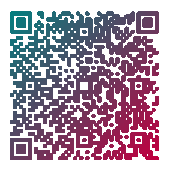
\includegraphics[width=3cm]{Cy_04_02_Application_02_Vehicule_qr}
\end{marginfigure}
\fi


\question{En supposant que les conditions initiales sont nulles, déterminer
l’expression numérique de la fonction de transfert $H_2(p)$ entre l’angle de lacet $\psi(p)$
et l’angle de braquage $\beta(p)$ de la roue avant : $H_2(p)=\dfrac{\psi(p)}{\beta(p)}$.
Discuter de la stabilité de ce modèle.}
\ifprof
\begin{corrige}
Dans le domaine de Laplace, on a 
$$
\left\{
\begin{array}{l}
211 p {\psi}(p)+225p{\alpha}(p)+840\alpha(p)=420\beta(p) \\
31p^2{\psi}(p)+91p{\psi}(p)-210\alpha(p)=420\beta(p) 
\end{array}
\right. $$

$
\Rightarrow \left\{
\begin{array}{l}
\left(225p+840\right)\alpha(p)=420\beta(p) - 211 p {\psi}(p)\\
\left(31p^2+91p\right){\psi}(p)-210\alpha(p)=420\beta(p) 
\end{array}
\right. $

$
\Rightarrow \left\{
\begin{array}{l}
\alpha(p)=\dfrac{420\beta(p) - 211 p {\psi}(p)}{225p+840}\\
\left(31p^2+91p\right){\psi}(p)-210\dfrac{420\beta(p) - 211 p {\psi}(p)}{225p+840}=420\beta(p) 
\end{array}
\right. $

$\left(31p^2+91p + \dfrac{210\times 211p}{225p+840}\right){\psi}(p)-210\dfrac{420\beta(p)}{225p+840}=420\beta(p) $

$\Rightarrow \left(31p^2+91p + \dfrac{210\times 211p}{225p+840}\right){\psi}(p)+\left(\dfrac{-210\times 420}{225p+840}-420\right)\beta(p)=0 $

$\Rightarrow H_2(p) = \dfrac{\dfrac{210\times 420}{225p+840}+420}{31p^2+91p + \dfrac{210\times 211p}{225p+840}} 
 = \dfrac{210\times 420+420\left(225p+840\right)}{\left(225p+840\right)\left(31p^2+91p \right)+ 210\times 211p}   $

$ = \dfrac{210\times 420+420\times 840+420\times 225p}{p\left(\left(225p+840\right)\left(31p+91 \right)+ 210\times 211\right)}   $


$ = \dfrac{210\times 420+420\times 840+420\times 225p}{p\left(225\times 31 p^2 
+840\times 31 p + 91 \times 225 p+91\times 840 + 210\times 211\right)}   $

$ = \dfrac{210\times 420+420\times 840+420\times 225p}{p\left(225\times 31 p^2 
+840\times 31 p + 91 \times 225 p+91\times 840 + 210\times 211\right)}   $

$ = \dfrac{441000+94500p}{p\left(6975  p^2 
+46515 p+120750\right)}   $
\end{corrige}
\else
\fi



